
\documentclass[a2,portrait]{a0poster}

\usepackage[T1]{fontenc}
\usepackage[ansinew]{inputenc} 
\usepackage{amsmath,amssymb} 

% Drop page numbers and section numbers.
\pagestyle{empty}
\setcounter{secnumdepth}{0}

% Include textpos package to position textblocks at arbitary 
% places on the page.
\usepackage[absolute]{textpos}

% Graphics and fonts
\usepackage{graphicx}
\usepackage{wrapfig,times}
\usepackage[footnotesize]{caption}

% Define some colors
\usepackage{color}
\definecolor{DarkBlue}{rgb}{0.0,0.0,0.5}
\definecolor{Red}{rgb}{0.9,0.0,0.1}

% see documentation for a0poster class for the size options here
\let\Textsize\normalsize
\def\Head#1{\noindent\hbox to \hsize{\hfil{\LARGE\color{DarkBlue} #1}}\bigskip}
\def\LHead#1{\noindent{\large\color{DarkBlue} #1}\smallskip}
\def\Subhead#1{\noindent{\large\color{DarkBlue} #1}}
\def\Title#1{{\LARGE\color{DarkBlue} #1}}

% Set up a grid and adjust the margins (in millimeters)
\TPGrid[15mm,15mm]{100}{150} 

% Adjust these parameters as you like
\parindent=0pt                  % paragraph indent
\parskip=10pt                    % space between paragraphs
\abovedisplayskip=10pt  % space above equations
\belowdisplayskip=10pt  % space below equations
\abovecaptionskip=0pt   % space between the image and the caption

% abbreviations
\newcommand{\ddd}{\,\mathrm{d}}








\begin{document} 


\small % font size options: \tiny, \scriptsize, \footnotesize, \small, \normalsize, \large, \Large, \LARGE, \huge, \Huge



% Title:
\begin{textblock}{100}(0,0)
\begin{center}
\Title{Poster Example}
\end{center}
\end{textblock}


%  Authors:
\begin{textblock}{100}(0,7)
\begin{center}
\small \bf Authors
\end{center}
\end{textblock}



% Block of text; the first parameter specifies the width of the block with respect to the grid defined by \TPGrid above,
% and the next two parameters give the coordinates of the left-hand upper corner of the block (with respect to the same grid):
\begin{textblock}{30}(0,20)
  \LHead{INTRODUCTION}
  
Consider the following linear inverse problem: given a vector $m$ and matrix $A$, find $x$ such that
\begin{equation} \label{eqn:IP} 
 Ax=m,
\end{equation}
where the matrix $A$ is ill-conditioned, i.e. its condition number is large.

This problem can be studied\ldots



\vspace{1cm}
\LHead{METHODS AND MATERIALS}

We shall solve \eqref{eqn:IP} using truncated SVD with trunctation level $\alpha>0$ as follows. \ldots


% Add an image here
\begin{figure}\centering
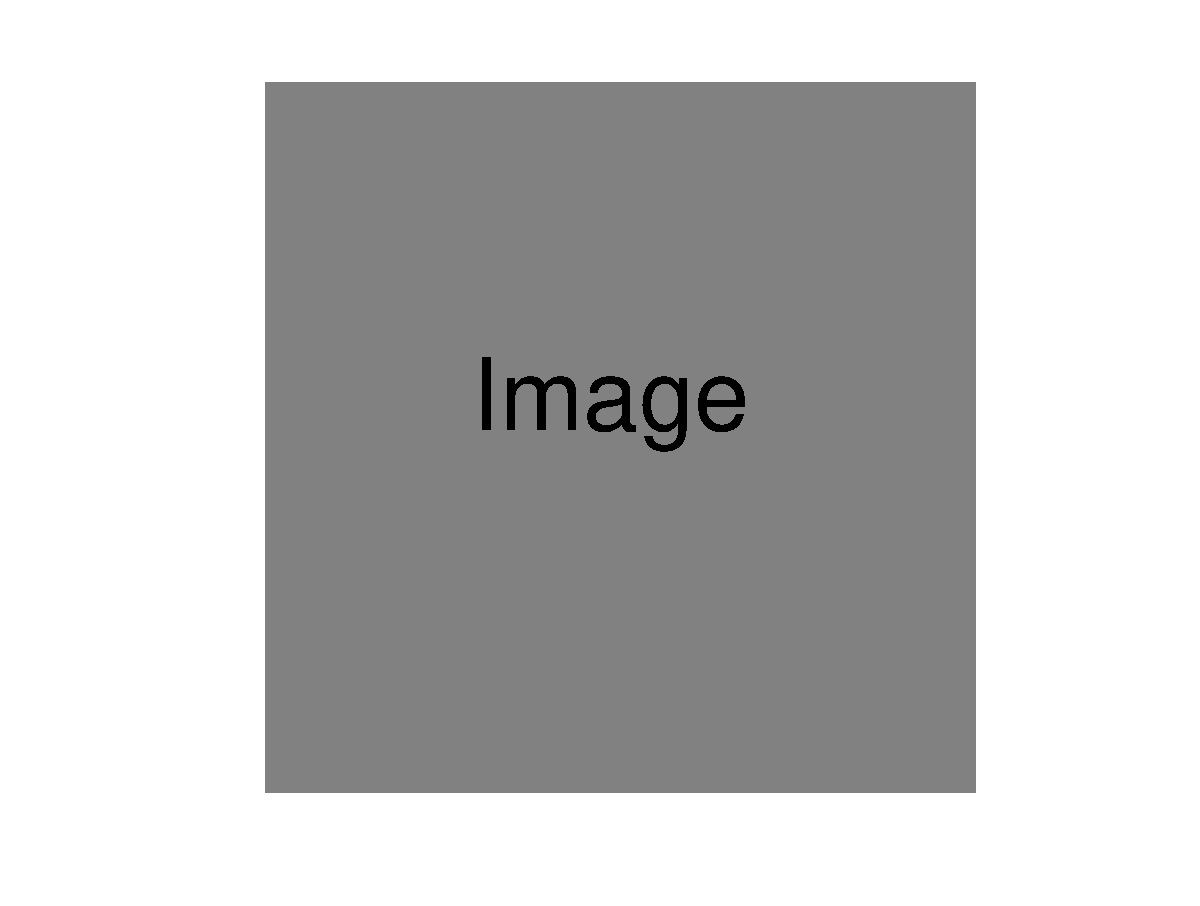
\includegraphics[width=10cm]{images/image.eps}
\caption{Example image.}
\label{fig:im1}
\end{figure}

As can be seen from Fig. \ref{fig:im1},\ldots


\end{textblock}











% Add another text block
\begin{textblock}{30}(35,50)

\LHead{RESULTS}

Present the numerical results\ldots

\end{textblock}






% You may also add wider blocks of text / figures:
\begin{textblock}{65}(35,20)

\begin{figure}
\begin{picture}(600,200)
\put(0,0){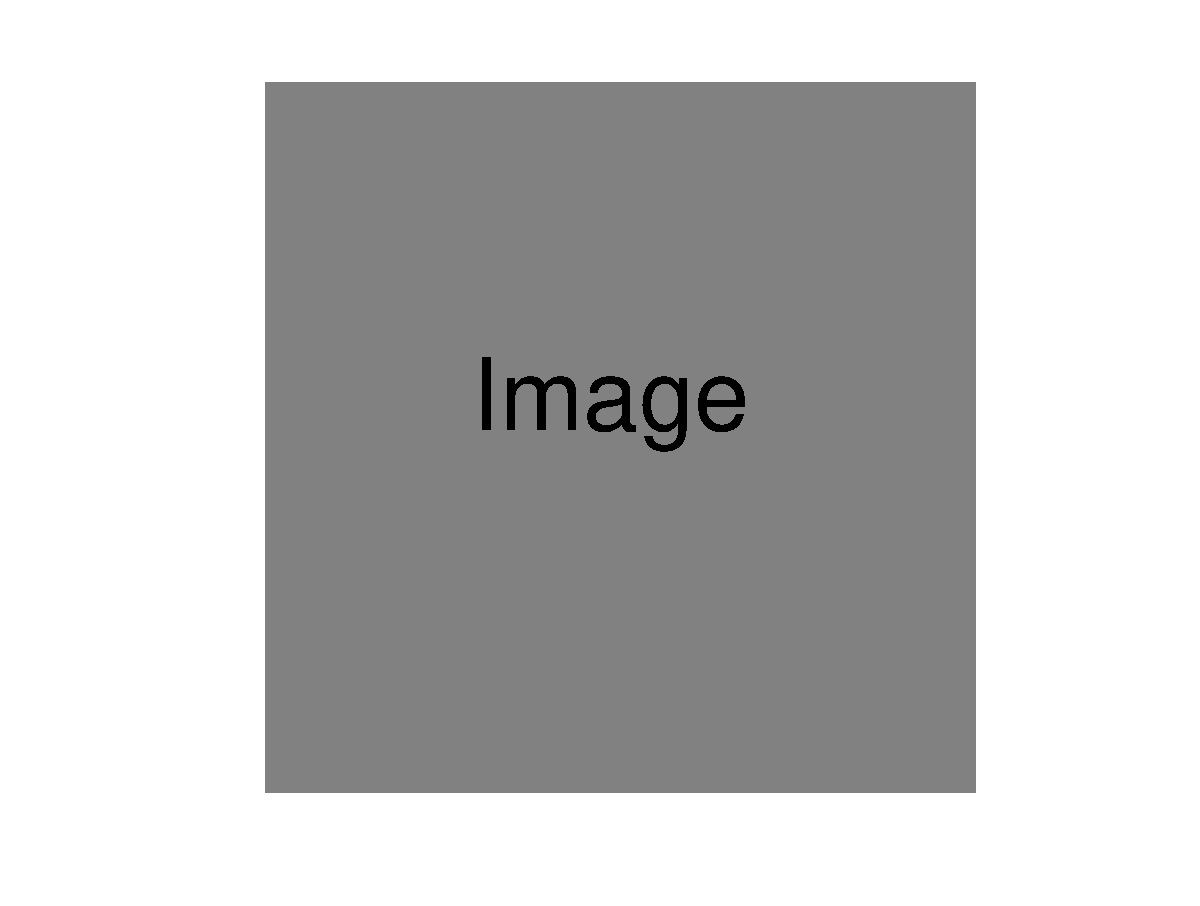
\includegraphics[width=300pt]{images/image.eps}}
\put(300,0){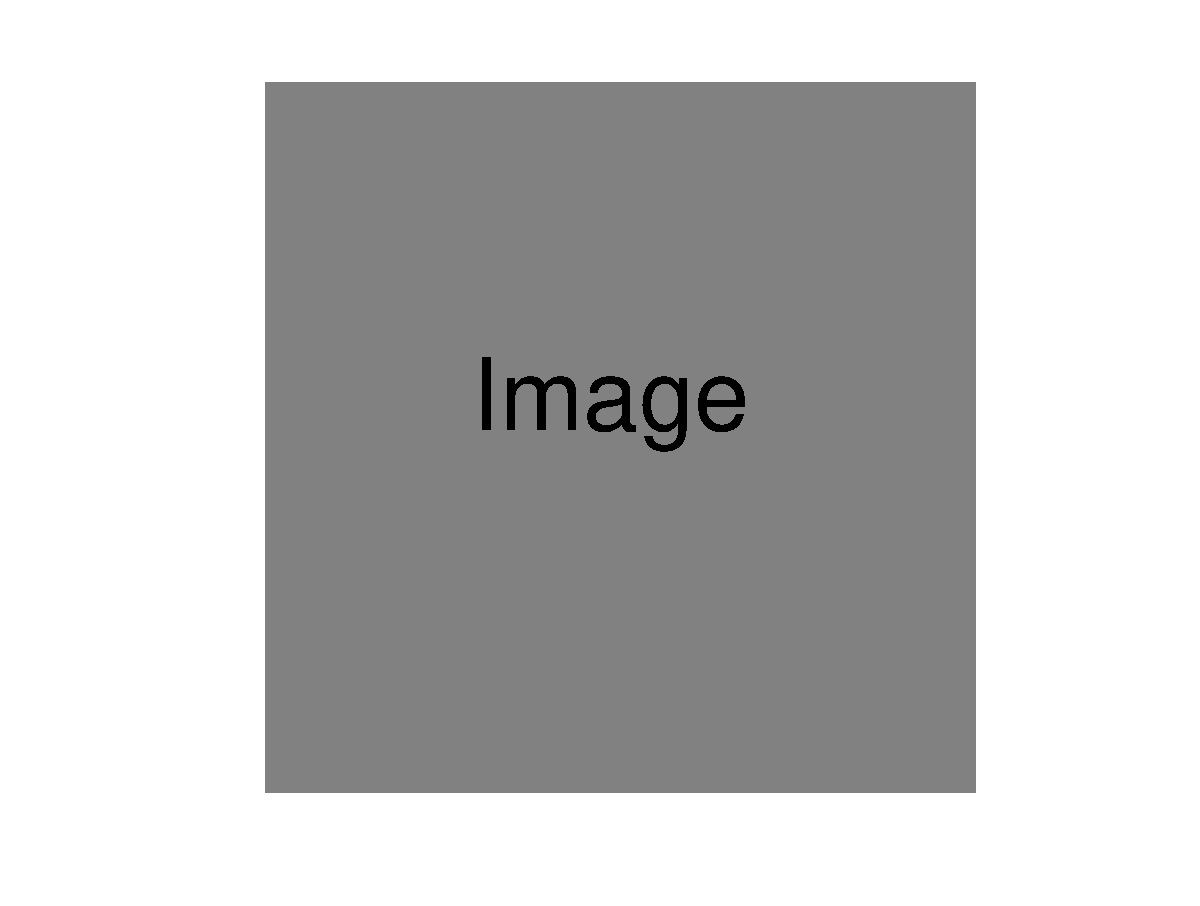
\includegraphics[width=300pt]{images/image.eps}}
\end{picture}
\caption{Some text can be added here\ldots}
\label{fig:images}
\end{figure}


\end{textblock}










\begin{textblock}{30}(70,80)

\LHead{DISCUSSION}

Discuss the results\ldots


\vspace{1cm}
{\bf References}  \\
\vspace{-1cm}

\footnotesize
{[1] Mueller J L and Siltanen S, {\em Linear and Nonlinear Inverse
Problems with Practical Applications}, SIAM 2012.}



\end{textblock}



\end{document}

